\chapter{Υλοποίηση}

Στο παρόν κεφάλαιο παρουσιάζεται η υλοποίηση του συστήματος,
όπως αυτή προέκυψε από τις σχεδιαστικές αποφάσεις του
Κεφαλαίου 4. Αρχικά παρουσιάζονται τα εργαλεία και οι
τεχνολογίες που επιλέχθηκαν, και στη συνέχεια αναλύονται
διαδοχικά τα τέσσερα βασικά στρώματα του συστήματος:
το \en{pipeline} επεξεργασίας γεωγραφικών δεδομένων,
η υλοποίηση των πρακτόρων, το \en{REST API} και το
\en{web frontend}.

\section{Εργαλεία και Τεχνολογίες}

Η υλοποίηση του συστήματος βασίζεται αποκλειστικά σε ανοιχτού
κώδικα εργαλεία και βιβλιοθήκες. Στο επίπεδο του \en{backend},
η γλώσσα προγραμματισμού \en{Python} αποτέλεσε την κύρια
επιλογή λόγω του πλούσιου οικοσυστήματος βιβλιοθηκών για
επιστημονικό υπολογισμό, γεωγραφικά δεδομένα και
μοντελοποίηση πρακτόρων.

Για την υλοποίηση του \en{ABM} χρησιμοποιήθηκε το
\en{framework Mesa}, το οποίο παρέχει τις βασικές αφαιρέσεις
για πράκτορες, μοντέλα και χώρους, όπως αναλύθηκε στην
Ενότητα 2.2. Ο χώρος κίνησης των πρακτόρων υλοποιείται μέσω
του \en{ContinuousSpace} του \en{Mesa}, που επιτρέπει
τοποθέτηση και μετακίνηση σε συνεχή δισδιάστατο χώρο με
μετρικές αποστάσεις.

Για την επεξεργασία γεωγραφικών δεδομένων χρησιμοποιήθηκαν
οι βιβλιοθήκες \en{GeoPandas} και \en{Shapely}, ενώ για τη
μετατροπή συντεταγμένων μεταξύ γεωγραφικών συστημάτων αναφοράς
η βιβλιοθήκη \en{PyProj}. Η κατασκευή και διαχείριση του γράφου
οδικού δικτύου υλοποιήθηκε με τη βιβλιοθήκη \en{NetworkX}, όπως
αναλύθηκε στην Ενότητα 2.4.3. Το \en{REST API} εκθέτεται μέσω
του \en{framework FastAPI}, το οποίο επιλέχθηκε για την υψηλή
του απόδοση και τη διαισθητική δήλωση \en{endpoints}.

Στο επίπεδο του \en{frontend}, η οπτικοποίηση του χάρτη
υλοποιείται με τη βιβλιοθήκη \en{Leaflet.js}, που παρέχει
διαδραστικό χάρτη βασισμένο σε \en{tiles} του
\en{OpenStreetMap}. Τα γραφήματα κατανομών υλοποιούνται με
τη βιβλιοθήκη \en{Chart.js}. Και οι δύο βιβλιοθήκες
εκτελούνται αποκλειστικά στον \en{browser}, χωρίς εξαρτήσεις
από εξωτερικά \en{frameworks}.

\section{\en{Pipeline} Φόρτωσης \en{GIS} Δεδομένων}

Το σύνολο της προεπεξεργασίας γεωγραφικών δεδομένων υλοποιείται
στη συνάρτηση \en{load\_gis\_model()} του αρχείου \en{main.py}.
Η συνάρτηση αυτή εκτελείται μία φορά κατά την εκκίνηση της
εφαρμογής και επιστρέφει όλα τα απαραίτητα δεδομένα για τη
δημιουργία του μοντέλου: τον γράφο οδικού δικτύου, τις
γεωμετρίες ακμών, τα \en{POI} και τα ξενοδοχεία.

Η συνάρτηση δέχεται ως παράμετρο το όνομα της πόλης
\en{(city\_name)}, το οποίο από προεπιλογή ορίζεται σε
$``$Πάτρα$"$. Η πόλη αναζητείται στο
\en{layer\ gis\_osm\_places\_free\_1} του αρχείου \en{Shapefile},
και σε περίπτωση πολλαπλών αποτελεσμάτων με το ίδιο όνομα
επιλέγεται αυτόματα η μεγαλύτερη σε πληθυσμό ή σημαντικότερη
κατηγορίας \en{(city $>$ town $>$ village)}. Γύρω από το κεντρικό
σημείο της πόλης δημιουργείται ζώνη αναφοράς \en{(buffer)}
ακτίνας 1.000 μέτρων στο σύστημα \en{EPSG:2100}, η οποία
μετατρέπεται σε ορθογώνιο πλαίσιο \en{(bounding box)} στο σύστημα
\en{WGS84}. Το πλαίσιο αυτό χρησιμοποιείται ως φίλτρο κατά τη
φόρτωση όλων των υπόλοιπων \en{layers} (οδοί, \en{POI}),
περιορίζοντας την ανάλυση αποκλειστικά στην περιοχή μελέτης και
μειώνοντας σημαντικά τον χρόνο επεξεργασίας.

\subsection{Φιλτράρισμα Οδών}

Από το \en{layer gis\_osm\_roads\_free\_1} φορτώνονται μόνο οι
οδοί εντός του \en{bounding box} της επιλεγμένης πόλης. Στη
συνέχεια εφαρμόζεται φίλτρο βάσει του πεδίου \en{fclass}, το
οποίο περιγράφει τον τύπο κάθε οδού. Διατηρούνται αποκλειστικά
οι κατηγορίες που επιτρέπουν πεζή κυκλοφορία: \en{footway, path,
pedestrian, steps, residential, living\_street, service,
unclassified, tertiary, secondary} και \en{primary}. Οδοί ταχείας
κυκλοφορίας \en{(motorway, trunk)} και σιδηροδρομικές γραμμές
αποκλείονται πλήρως.

Μετά το φιλτράρισμα, οι γεωμετρίες μετατρέπονται στο σύστημα
συντεταγμένων \en{EPSG:2100} (ΕΓΣΑ '87), το οποίο διατηρεί
αποστάσεις σε μέτρα. Αυτή η μετατροπή είναι απαραίτητη για τον
ακριβή υπολογισμό αποστάσεων και ταχυτήτων κατά την κίνηση των
πρακτόρων. Εάν ο αριθμός των φιλτραρισμένων οδών υπερβαίνει το
όριο των 5.000 τμημάτων, το σύστημα ζητά επιβεβαίωση από τον
χρήστη, καθώς η κατασκευή του γράφου για τόσο μεγάλο δίκτυο
απαιτεί σημαντικό υπολογιστικό χρόνο.

\subsection{Κατασκευή Γράφου}

Η κατασκευή του γράφου από τα ακατέργαστα τμήματα οδών είναι το
υπολογιστικά εντατικότερο βήμα του \en{pipeline} και υλοποιείται
σε τρεις φάσεις.

Στην πρώτη φάση εντοπίζονται τα σημεία τομής μεταξύ τμημάτων οδών.
Για κάθε ζεύγος τμημάτων ελέγχεται αν τέμνονται γεωμετρικά. Τα
άκρα όλων των τμημάτων (αρχή και τέλος κάθε \en{LineString})
προστίθενται αυτόματα ως υποψήφια σημεία κόμβων. Τα σημεία τομής
που δεν συμπίπτουν με άκρο (εσωτερικές τομές) εντοπίζονται και
καταγράφονται κι αυτά ως υποψήφια σημεία κόμβων.

Στη δεύτερη φάση δημιουργούνται οι κόμβοι του γράφου. Κάθε
μοναδικό σημείο τομής μετατρέπεται σε κόμβο με μοναδικό
αναγνωριστικό. Για την αντιμετώπιση της γεωμετρικής ανακρίβειας
των δεδομένων \en{OSM}, εφαρμόζεται τεχνική \en{snapping}, όπου
συντεταγμένες που απέχουν λιγότερο από 5 μέτρα στρογγυλοποιούνται
στο πλησιέστερο πολλαπλάσιο του 5, ώστε να αντιστοιχιστούν στον
ίδιο κόμβο. Χωρίς αυτή την τεχνική, μικρές αριθμητικές αποκλίσεις
στα δεδομένα θα δημιουργούσαν χιλιάδες διπλότυπους κόμβους και
αποσυνδεδεμένα τμήματα δικτύου.

Στην τρίτη φάση κάθε τμήμα οδού διασπάται στα σημεία που
εντοπίστηκαν κοντά του (εντός \en{snap tolerance}). Για κάθε τμήμα
υπολογίζεται η προβολή κάθε κόμβου πάνω στη γραμμή, και το τμήμα
διασπάται σε υποτμήματα μεταξύ διαδοχικών προβολών. Κάθε υποτμήμα
αποθηκεύεται ως ακμή του γράφου με τη γεωμετρία του
\en{(LineString)} και αντίστοιχη αντίστροφη γεωμετρία για την
κίνηση προς αμφότερες τις κατευθύνσεις.

\begin{figure}[H] \centering
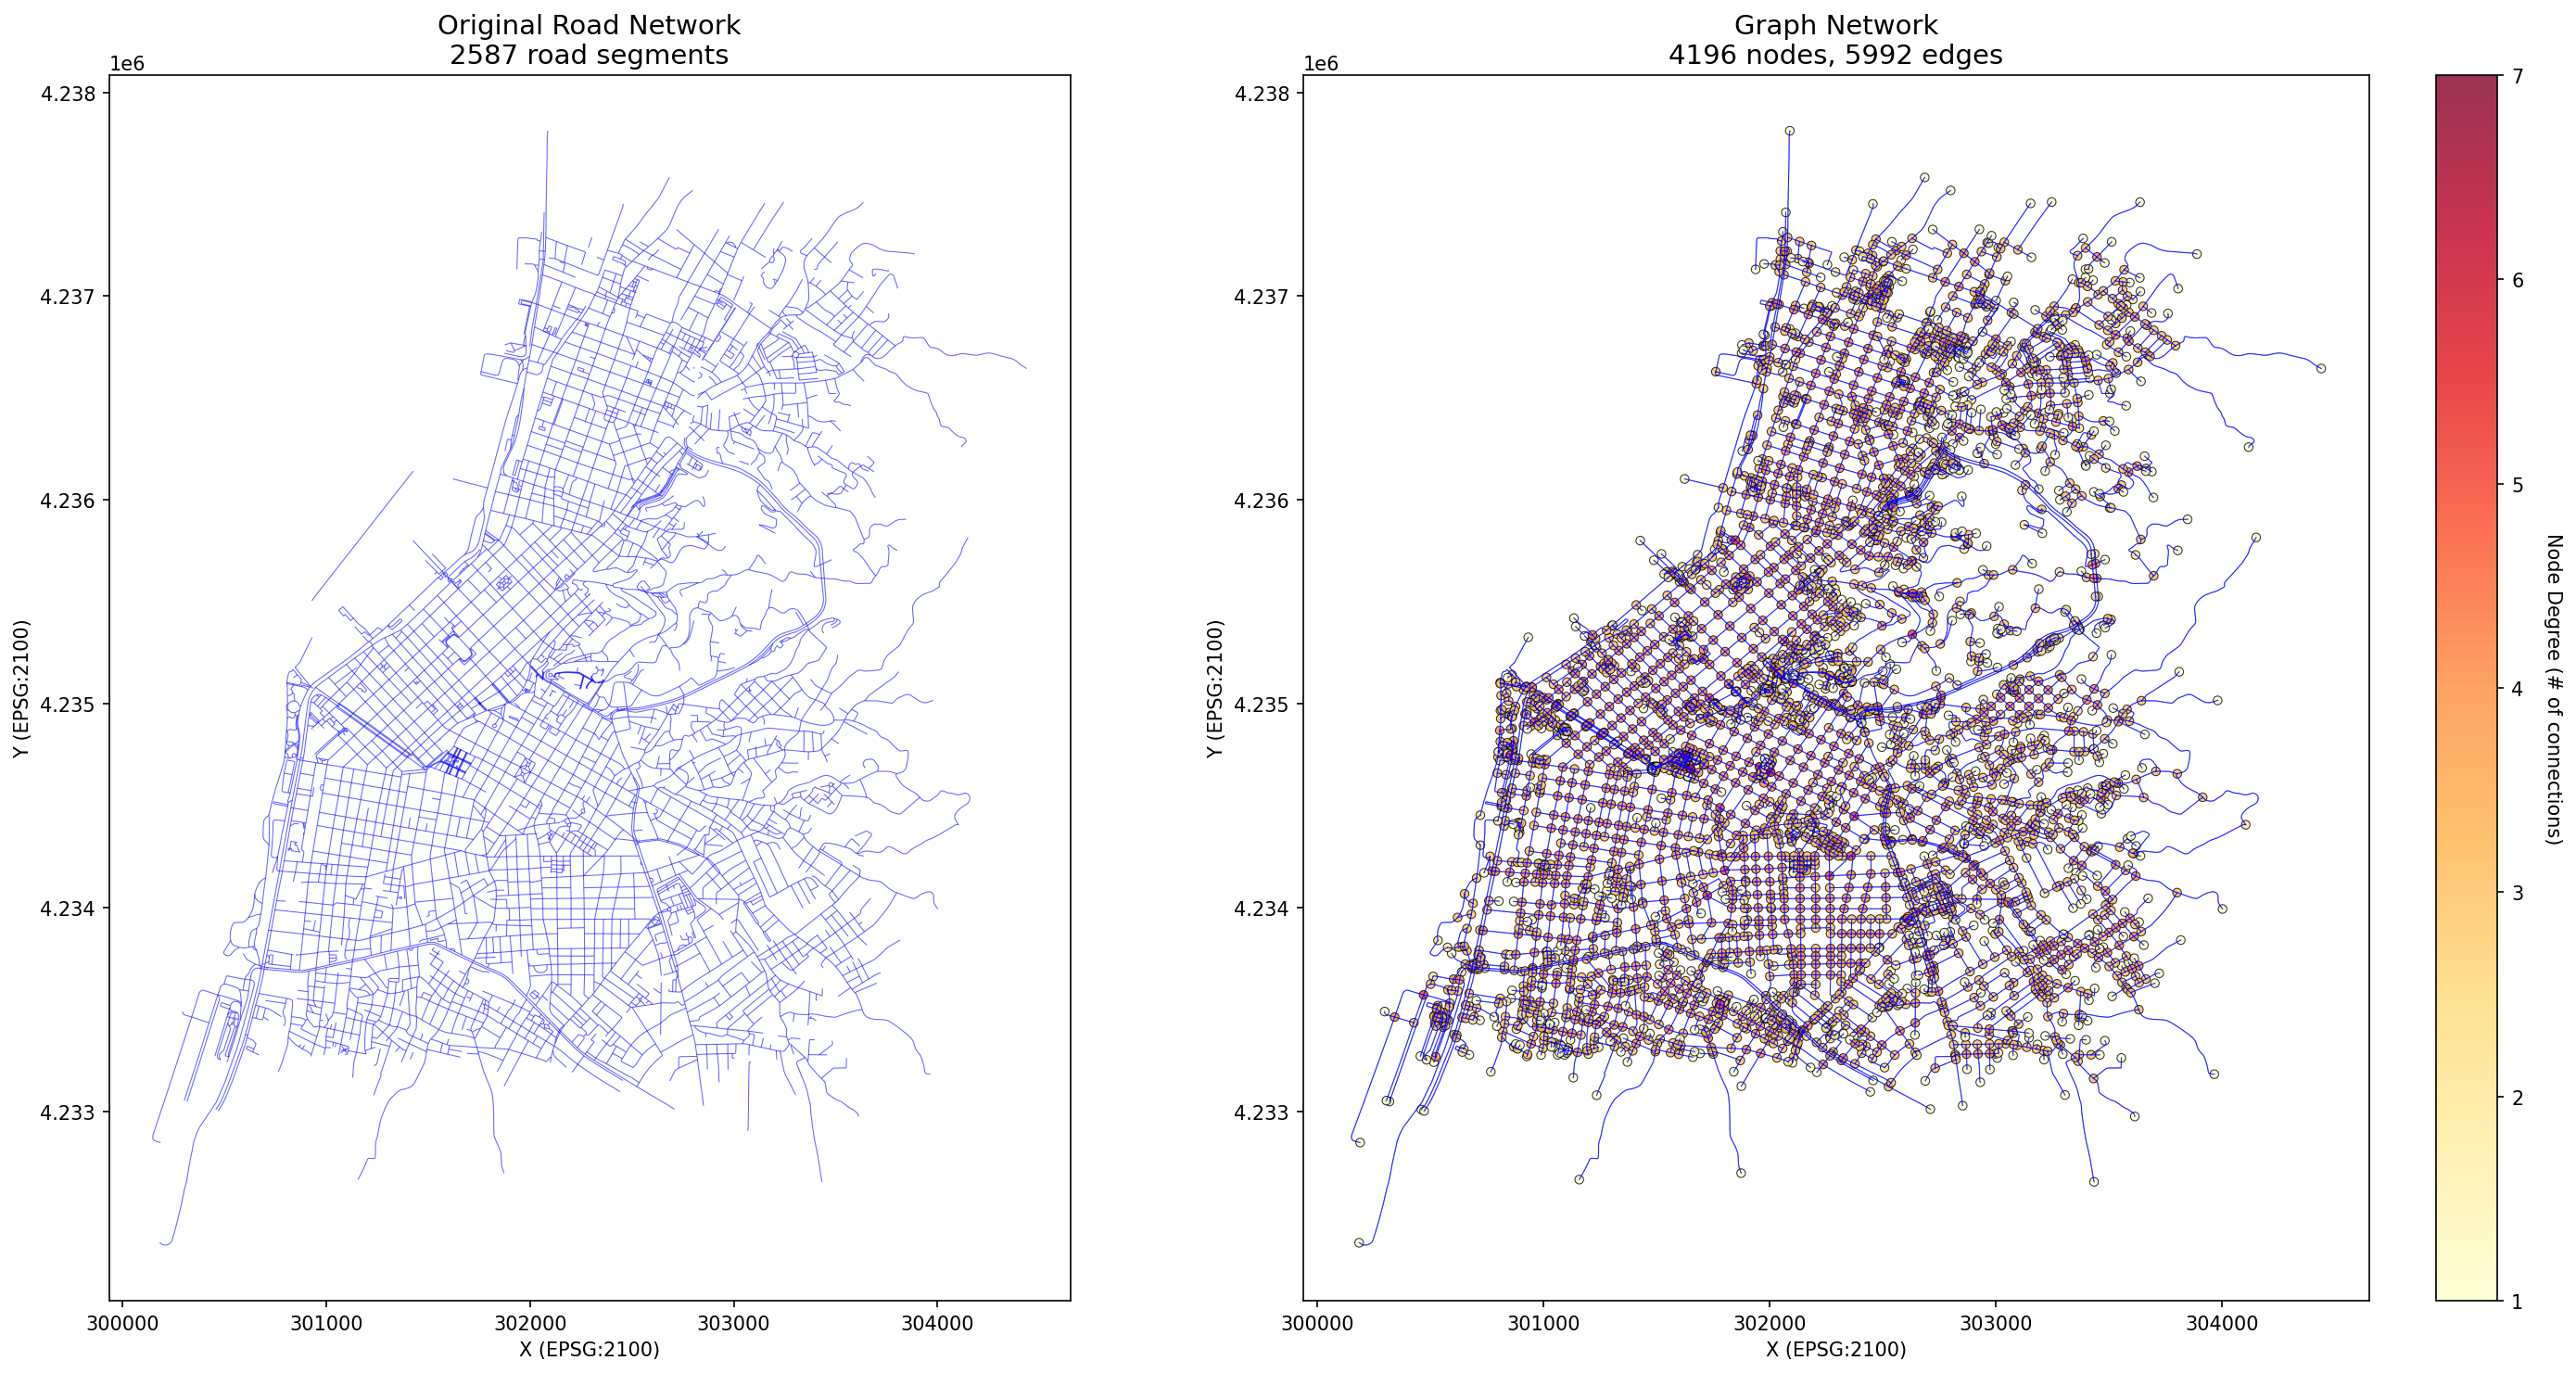
\includegraphics[width=\textwidth]{static/figures/road_network_graph.png}
\caption{Κατασκευή Γράφου Οδικού Δικτύου}\label{road_network_graph}
\end{figure}

\subsection{Ελκυστικότητα Δρόμων}

Μετά την κατασκευή του γράφου, κάθε ακμή αποκτά βαθμολογία
ελκυστικότητας \en{(attractiveness score)} που χρησιμοποιείται
από τον αλγόριθμο πλοήγησης των τουριστών. Η βαθμολογία
υπολογίζεται ως άθροισμα δύο συνιστωσών.

Η πρώτη συνιστώσα είναι η βασική βαθμολογία τύπου οδού
\en{(base score)}, όπου: \en{pedestrian=5, footway=4,
living\_street=3, residential=2, tertiary/secondary/primary=1.}
Οι πεζόδρομοι λαμβάνουν υψηλότερη βαθμολογία γιατί είναι φυσικά
πιο ελκυστικοί για τους πεζούς τουρίστες.

Η δεύτερη συνιστώσα είναι η βαθμολογία \en{POI (poi score)}, όπου
για κάθε ακμή δημιουργείται \en{buffer} 30 μέτρων και
καταμετρούνται τα \en{POI} που περιέχονται σε αυτή. Κάθε
\en{POI Tier A} συνεισφέρει 10 μονάδες, κάθε \en{Tier B} 3 μονάδες
και κάθε \en{Tier C} 1 μονάδα. Η τελική βαθμολογία είναι το
άθροισμα \en{base score} και \en{poi score}, και αποθηκεύεται ως
χαρακτηριστικό της ακμής στον γράφο.

\subsection{Φόρτωση \en{POI} και Ξενοδοχείων}

Τα σημεία ενδιαφέροντος φορτώνονται από το
\en{layer gis\_osm\_pois\_free\_1} εντός του \en{bounding box}
της πόλης. Για κάθε \en{POI} εξετάζεται το πεδίο \en{fclass} και
κατατάσσεται στο αντίστοιχο \en{tier}:
\begin{itemize}
\item \en{Tier A} για μουσεία, αξιοθέατα, μνημεία, αρχαιολογικούς
χώρους, κάστρα, πάρκα θεματικής αναψυχής και εμπορικά κέντρα
\item \en{Tier B} για καφετέριες, εστιατόρια, \en{fast food, bar}
και \en{pub}
\item \en{Tier C} για καταστήματα ρουχισμού, βιβλιοπωλεία,
αρτοποιεία, σούπερ μάρκετ και δώρα.
\end{itemize}
\en{POI} που δεν ανήκουν σε κανέναν από τους παραπάνω τύπους
αγνοούνται. Κάθε \en{POI} αποθηκεύεται ως λεξικό με μοναδικό
αναγνωριστικό, όνομα, γεωμετρία, τύπο \en{fclass} και \en{tier}.

Τα ξενοδοχεία αναζητούνται στο ίδιο \en{layer} με τύπους
\en{hotel, hostel, motel} και \en{guest\_house}. Εάν εντοπιστούν
λιγότερα από 3, το σύστημα επεκτείνει αναζήτηση σε \en{POI} τύπου
\en{accommodation} και στη συνέχεια, αν χρειαστεί, χρησιμοποιεί
τα πρώτα διαθέσιμα \en{POI} υψηλής επισκεψιμότητας (εστιατόρια,
καφετέριες, αξιοθέατα) ως υποκατάστατα. Αυτή η λογική εναλλακτικής
αναζήτησης εξασφαλίζει τη λειτουργία του μοντέλου ακόμα και για
πόλεις με ελλιπή καταγραφή ξενοδοχείων στα δεδομένα \en{OSM}.

\section{Υλοποίηση Πρακτόρων}

Οι πράκτορες υλοποιούνται στο αρχείο \en{agents.py}. Η κλάση
\en{ResidentAgent} κληρονομεί από την \en{Agent} του \en{Mesa}
και υλοποιεί απλή λογική ενημέρωσης ευτυχίας. Η κλάση
\en{TouristAgent} κληρονομεί επίσης από \en{Agent} και υλοποιεί
το σύνολο της σύνθετης συμπεριφοράς που περιγράφηκε στην
Ενότητα 4.4.2. Και οι δύο κλάσεις ενσωματώνονται στην κλάση
\en{CityModel}, η οποία κληρονομεί από \en{Model} του \en{Mesa}
και διαχειρίζεται τον χρόνο, τον χώρο και την ενεργοποίηση των
πρακτόρων.

\subsection{Ημερήσιος Κύκλος Τουρίστα}

Ο ημερήσιος κύκλος του τουρίστα υλοποιείται στη μέθοδο \en{step()}
της \en{TouristAgent}, η οποία καλείται σε κάθε βήμα προσομοίωσης
(10 λεπτά). Η λογική βασίζεται στον τρέχοντα χρόνο της
προσομοίωσης \en{(current\_hour, current\_min)} και στην εσωτερική
μεταβλητή κατάστασης \en{state}.

Κατά τις ώρες 00:00–08:00, εάν ο τουρίστας δεν βρίσκεται ήδη σε
κατάσταση \en{sleeping}, μεταφέρεται στο ξενοδοχείο του (μέθοδος
\en{teleport\_to\_hotel()}) και η κατάστασή του ορίζεται σε
\en{sleeping}. Η ικανοποίησή του επαναφέρεται στην αρχική τιμή
0.7. Στις 8:00 π.μ., εάν η κατάσταση είναι \en{sleeping}, καλείται
η μέθοδος \en{\_initialize\_daily\_targets()} που σαρώνει ακτίνα
100 μέτρων για \en{POI} και ορίζει τον πρώτο στόχο της ημέρας.

Κατά τις ενεργές ώρες, ο τουρίστας βρίσκεται σε μία από τις εξής
καταστάσεις: \en{walking\_to\_tier\_a, walking\_to\_tier\_b,
walking\_to\_tier\_c} (μετάβαση προς \en{POI}),
\en{visiting\_tier\_a, visiting\_tier\_b, visiting\_tier\_c}
(παραμονή σε \en{POI}), ή \en{casual\_wandering} (ελεύθερη
περιπλάνηση χωρίς στόχο). Η διάρκεια επίσκεψης ορίζεται ως
180 λεπτά για \en{Tier A}, 60 λεπτά για \en{Tier B} και
20 λεπτά για \en{Tier C}. Τα \en{POI Tier A} δέχονται επισκέπτες
μέχρι τις 18:00 και κλείνουν στις 20:00. Κατά τα μεσάνυχτα,
η μέθοδος \en{\_reset\_daily\_attributes()} του \en{CityModel}
επαναφέρει την ευτυχία κατοίκων, την ικανοποίηση τουριστών και
τις πιθανότητες παρεκτροπής σε αρχικές τιμές.

\begin{figure}[H] \centering
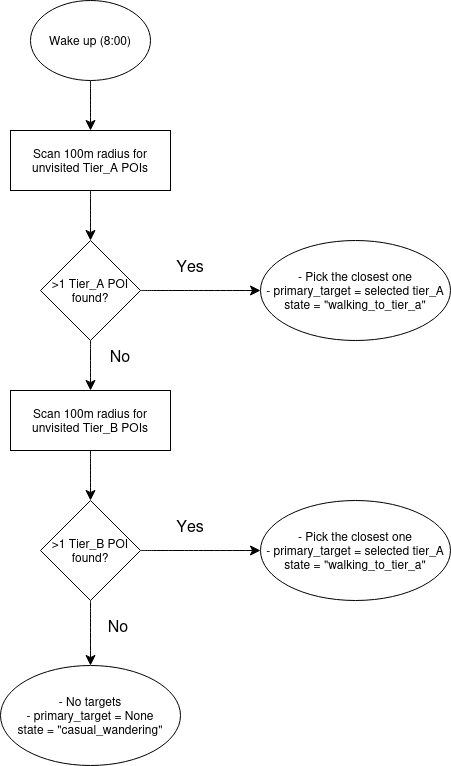
\includegraphics[width=0.5\textwidth]{static/figures/wake_up.png}
\caption{Επιλογή Στόχου κατά το Ξύπνημα}\label{wake_up}
\end{figure}

\subsection{\en{Forward Vision Scan} και \en{Detour} Λογική}

Ο μηχανισμός \en{forward vision scan} υλοποιείται στη μέθοδο 
\en{\_forward\_vision\_scan()}, η οποία καλείται σε κάθε βήμα
όταν ο τουρίστας βρίσκεται σε κατάσταση μετάβασης προς
\en{POI}. Η μέθοδος αναζητάει ανεπίσκεπτα \en{POI Tier B} ή \en{C}
που βρίσκονται εντός ακτίνας 30 μέτρων από την τρέχουσα θέση του
τουρίστα.

Για λόγους απόδοσης, κατά την εκκίνηση του μοντέλου κατασκευάζεται
μία δομή \en{KDTree (scipy.spatial.KDTree)} πάνω στις συντεταγμένες
όλων των \en{POI}. Αντί να επαναλαμβάνεται πλήρης σάρωση όλων των
\en{POI} σε κάθε βήμα και για κάθε τουρίστα, το \en{KDTree}
επιτρέπει ανάκτηση μόνο των \en{POI} εντός της επιθυμητής ακτίνας
σε \en{O(log n)} χρόνο, μειώνοντας σημαντικά το υπολογιστικό κόστος
κατά την εκτέλεση της προσομοίωσης.

Έπειτα, για κάθε \en{POI} εντός ακτίνας υπολογίζεται η γωνία μεταξύ
της κατεύθυνσης προς τον τρέχοντα στόχο και της κατεύθυνσης προς το
\en{POI}, μέσω εσωτερικού γινομένου \en{(dot product)} των
αντίστοιχων μοναδιαίων διανυσμάτων. Εάν η γωνία είναι μικρότερη
από 30 μοίρες, το \en{POI} βρίσκεται εντός του οπτικού κώνου και
καλείται η μέθοδος \en{\_consider\_poi\_detour()}.

Η μέθοδος \en{\_consider\_poi\_detour()} αποφασίζει στοχαστικά αν
θα γίνει παρεκτροπή, η οποία συμβαίνει με πιθανότητα 30\% για
\en{POI Tier B} και 20\% για \en{Tier C}. Σε περίπτωση
παρεκτροπής, ο τρέχων πρωτεύων στόχος αποθηκεύεται ως δευτερεύων
\en{(secondary\_target)} και το \en{POI} ορίζεται ως νέος
πρωτεύων στόχος. Μετά την ολοκλήρωση της επίσκεψης, η μέθοδος
\en{\_exit\_poi()} ελέγχει αν ο δευτερεύων στόχος βρίσκεται εντός
300 μέτρων. Aν ναι, αποκαθίσταται ως πρωτεύων στόχος, αλλιώς ο
τουρίστας περνά σε κατάσταση \en{casual\_wandering}. Μετά από
κάθε επίσκεψη, η αντίστοιχη πιθανότητα παρεκτροπής μειώνεται
κατά 0.15 για \en{Tier B} (ελάχιστο 0.15) και 0.05 για
\en{Tier C} (ελάχιστο 0.05).

\begin{figure}[H] \centering
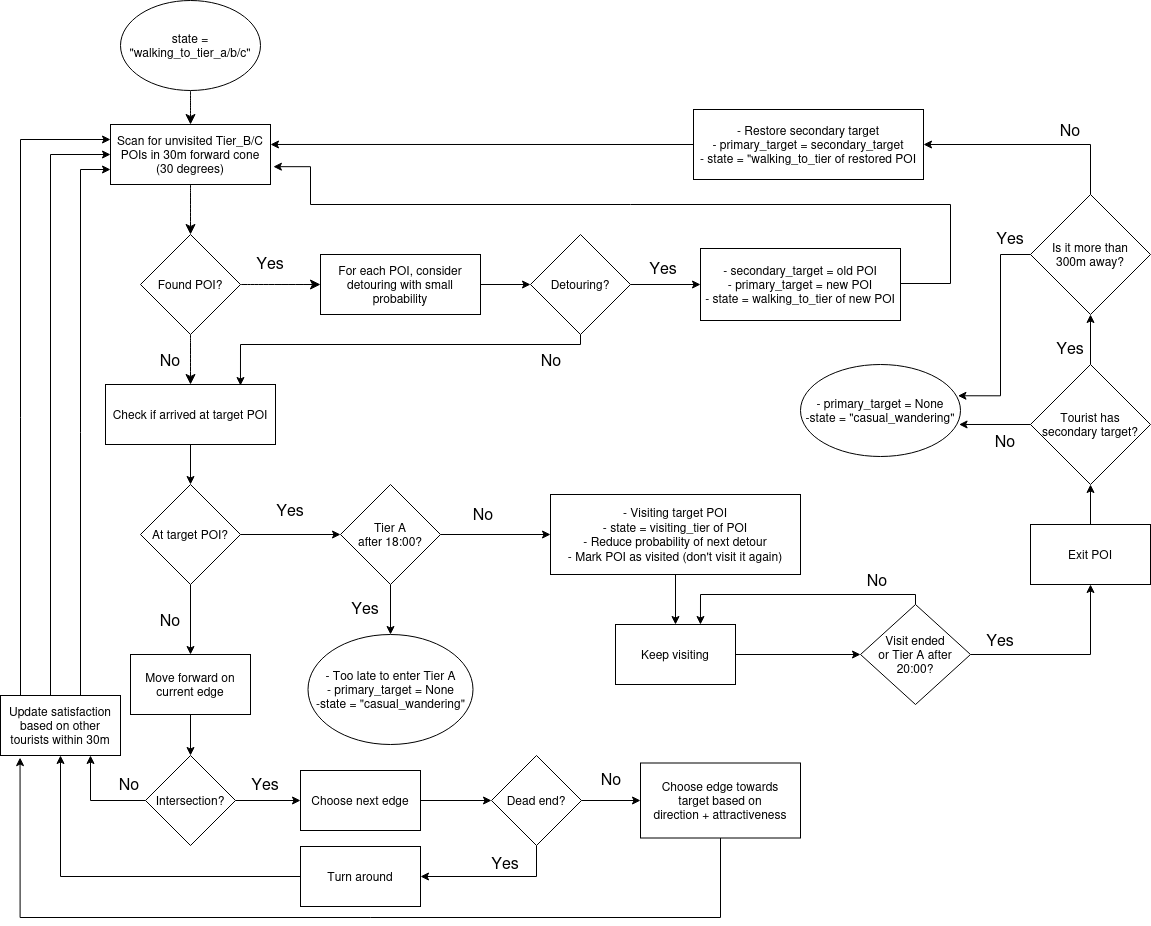
\includegraphics[width=\textwidth]{static/figures/walking_to_tier.png}
\caption{Βασικό Διάγραμμα Ροής}\label{walking_to_tier-100-23r}
\end{figure}

\begin{figure}[H] \centering
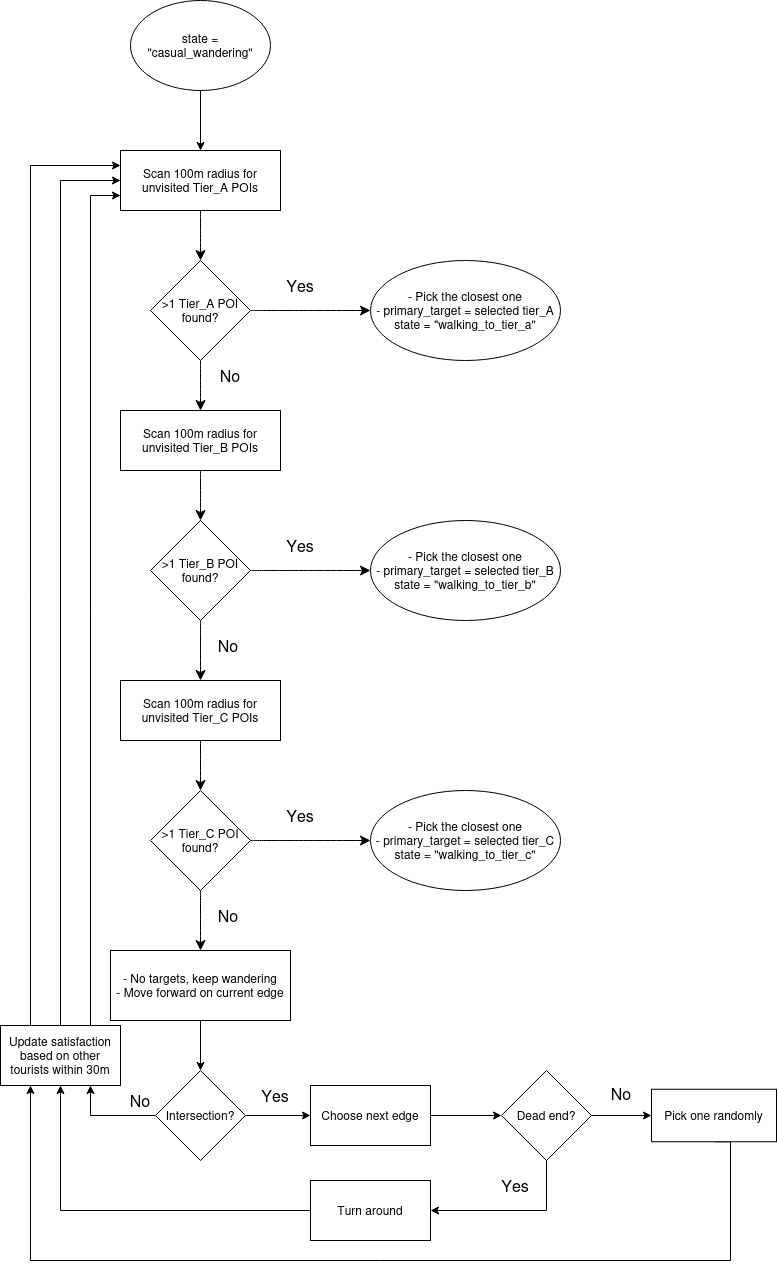
\includegraphics[width=0.8\textwidth]{static/figures/casual_wandering.png}
\caption{Περίπτωση Περιπλάνησης}\label{casual_wandering}
\end{figure}

\subsection {Υβριδική Εύρεση Διαδρομής}

Η κίνηση πάνω στο γράφο υλοποιείται στη μέθοδο
\en{\_move\_on\_graph()}. Σε κάθε βήμα, ο τουρίστας προχωρά κατά
\en{speed} μέτρα πάνω στην τρέχουσα ακμή
\en{(pos\_on\_edge += speed)}. Όταν η \en{pos\_on\_edge} υπερβεί
το μήκος της ακμής, ο τουρίστας έχει φτάσει στον επόμενο κόμβο και
καλείται η μέθοδος \en{\_choose\_next\_edge()}. Η τρέχουσα θέση
στον χώρο υπολογίζεται με γεωμετρική παρεμβολή πάνω στη
\en{LineString} της ακμής (μέθοδος \en{interpolate} της
\en{Shapely}) και μετατρέπεται σε συντεταγμένες μοντέλου.

Η επιλογή επόμενης ακμής υλοποιείται στη μέθοδο
\en{\_choose\_next\_edge()}. Εάν ο τουρίστας δεν έχει ενεργό
στόχο, επιλέγει τυχαία μεταξύ των διαθέσιμων γειτονικών κόμβων
(αποφεύγοντας άμεση επιστροφή). Εάν έχει στόχο, καλείται η
μέθοδος \en{\_choose\_edge\_toward\_target()}.

Στη μέθοδο \en{\_choose\_edge\_toward\_target()} κάθε γειτονικός
κόμβος βαθμολογείται ως εξής: υπολογίζεται η ευθυγράμμιση
\en{(alignment)} ως \en{dot product} μεταξύ του μοναδιαίου
διανύσματος προς τον στόχο και του μοναδιαίου διανύσματος προς τον
γείτονα, ενώ αρνητικές τιμές (οπισθοδρόμηση) μηδενίζονται.
Η τελική βαθμολογία υπολογίζεται ως: \en{score = alignment × 0.8 +
(attractiveness / 10) × 0.2} όταν ο στόχος απέχει άνω των
200 μέτρων (μακρινός στόχος), και \en{score = alignment ×
attractiveness} όταν είναι κοντά. Η επιλογή γίνεται πιθανοτικά
βάσει των κανονικοποιημένων βαθμολογιών, με πιθανότητα τυχαίας
εξερεύνησης 5\% για μακρινό στόχο και 15\% για κοντινό.

\subsection{Μετρικές Ευτυχίας και Ικανοποίησης}

Η ευτυχία των κατοίκων ενημερώνεται στη μέθοδο
\en{\_update\_happiness()} της \en{ResidentAgent}. Σε κάθε βήμα
κατά τις ώρες κινητικότητας (8:00–24:00), μετράται ο αριθμός τουριστών
εντός ακτίνας 30 μέτρων μέσω της μεθόδου \en{get\_neighbors()} του
\en{ContinuousSpace}. Οι κανόνες ενημέρωσης είναι: +0.02 εάν δεν
υπάρχουν τουρίστες, +0.005 για 1–3 τουρίστες, -0.01 για 4–10
τουρίστες, -0.03 για άνω των 10. Η τιμή περιορίζεται πάντα στο
διάστημα [0.0, 1.0].

Η ικανοποίηση των τουριστών ενημερώνεται με αντίστοιχο τρόπο στη
μέθοδο \en{\_update\_satisfaction()} της \en{TouristAgent} μετά από
κάθε βήμα κίνησης. Με τον ίδιο μηχανισμό \en{get\_neighbors()}
καταμετρούνται οι γειτονικοί τουρίστες εντός 30 μέτρων: η ικανοποίηση
αυξάνεται κατά +0.01 εάν υπάρχουν έως 5 τουρίστες, παραμένει
αμετάβλητη για 6–15, και μειώνεται κατά -0.02 για άνω των 15.
Και αυτή η τιμή περιορίζεται στο [0.0, 1.0].

Η παραγωγή των \en{heatmaps} υλοποιείται στη μέθοδο
\en{generate\_heatmap()} του \en{CityModel}. Ο χώρος διαιρείται σε
πλέγμα κελιών 10×10 μέτρων. Για κάθε ενεργό τουρίστα (εκτός κατάστασης
\en{sleeping}), προστίθεται η τιμή \en{noise} ή \en{pollution} στο
κελί που βρίσκεται, και το 30\% της τιμής στα 8 γειτονικά κελιά,
προσομοιώνοντας τη χωρική διάχυση του θορύβου και της ρύπανσης.

\section{\en{REST API}}

Το \en{REST API} υλοποιείται με \en{FastAPI} στο αρχείο \en{main.py}.
Κατά την εκκίνηση \en{(startup event)}, καλείται η
\en{load\_gis\_model()} και δημιουργείται το \en{CityModel}. Το
μοντέλο αποθηκεύεται σε καθολική μεταβλητή και είναι προσβάσιμο από
όλα τα \en{endpoints}. Τα αρχεία του \en{frontend} σερβίρονται ως
στατικά αρχεία από τον φάκελο \en{static/}.

Το \en{endpoint GET /state} επιστρέφει την πλήρη κατάσταση της
προσομοίωσης, δηλαδή τον τρέχοντα χρόνο, τη λίστα όλων των πρακτόρων
με θέση και χαρακτηριστικά, τη λίστα ξενοδοχείων και τη λίστα \en{POI}.
Οι συντεταγμένες μετατρέπονται από \en{EPSG}:2100 σε \en{WGS84}
(γεωγραφικό πλάτος/μήκος) μέσω του \en{Transformer} της \en{PyProj},
ώστε να είναι απευθείας χρησιμοποιήσιμες από το \en{Leaflet.js}.

Το \en{endpoint POST /step} εκτελεί ένα βήμα προσομοίωσης
\en{(model.step())} και επιστρέφει την ενημερωμένη κατάσταση των
πρακτόρων. Το \en{endpoint POST /skip\_to\_morning} καλεί τη μέθοδο
\en{skip\_to\_morning()} του μοντέλου, η οποία ορίζει τον χρόνο σε
08:00, τηλεμεταφέρει όλους τους τουρίστες στα ξενοδοχεία τους και
επαναφέρει τις μεταβλητές ευημερίας. Τα \en{endpoints
GET /heatmap/noise} και \en{GET /heatmap/pollution} καλούν τη
\en{generate\_heatmap()} και επιστρέφουν το πλέγμα τιμών μαζί με
τις γεωγραφικές συντεταγμένες κάθε κελιού σε \en{WGS84}. Τα
\en{endpoints GET /distribution/happiness} και
\en{GET /distribution/satisfaction} επιστρέφουν ιστόγραμμα κατανομής
των αντίστοιχων μεταβλητών σε 10 \en{bins} του διαστήματος [0, 1].

\section{\en{Frontend} Οπτικοποίηση}

Το \en{frontend} υλοποιείται σε δύο αρχεία: \en{index.html} που
ορίζει τη δομή της σελίδας και φορτώνει τις εξαρτήσεις, και
\en{map.js} που περιέχει όλη τη λογική οπτικοποίησης και
αλληλεπίδρασης. Κατά τη φόρτωση της σελίδας, καλείται το
\en{endpoint /state} και αρχικοποιείται ο χάρτης με τις θέσεις
πρακτόρων, \en{POI} και ξενοδοχείων.

\subsection{Χάρτης \en{Leaflet} και \en{Layers}}

Ο χάρτης αρχικοποιείται κεντραρισμένος στην Πάτρα με \en{zoom level}
13. Ως υπόβαθρο χρησιμοποιούνται \en{tiles} του \en{OpenStreetMap}.
Τα δεδομένα οργανώνονται σε πέντε ανεξάρτητα \en{LayerGroups:
Residents, Tourists, Hotels, POIs} και \en{Heatmap}. Ο χρήστης
μπορεί να ενεργοποιεί ή να απενεργοποιεί κάθε \en{layer} ανεξάρτητα
μέσω του ενσωματωμένου \en{layer control} του \en{Leaflet}.

Οι κάτοικοι απεικονίζονται ως μπλε κύκλοι και οι τουρίστες ως
κόκκινοι κύκλοι \en{(CircleMarker)}. Κάθε πράκτορας φέρει \en{popup}
με τα πλήρη χαρακτηριστικά του. Για τους κατοίκους εμφανίζεται η
τιμή ευτυχίας, ενώ για τους τουρίστες εμφανίζονται θόρυβος, ρύπανση,
ικανοποίηση, τρέχουσα κατάσταση, πρωτεύων και δευτερεύων στόχος.
Τα ξενοδοχεία απεικονίζονται με μπλε \en{marker} και τα \en{POI}
με έγχρωμους \en{markers} διαφορετικού μεγέθους ανά \en{tier}
(πράσινος/μεγάλος για \en{Tier A}, κίτρινος/μεσαίος για \en{Tier B},
πορτοκαλί/μικρός για \en{Tier C}).

\begin{figure}[H] \centering
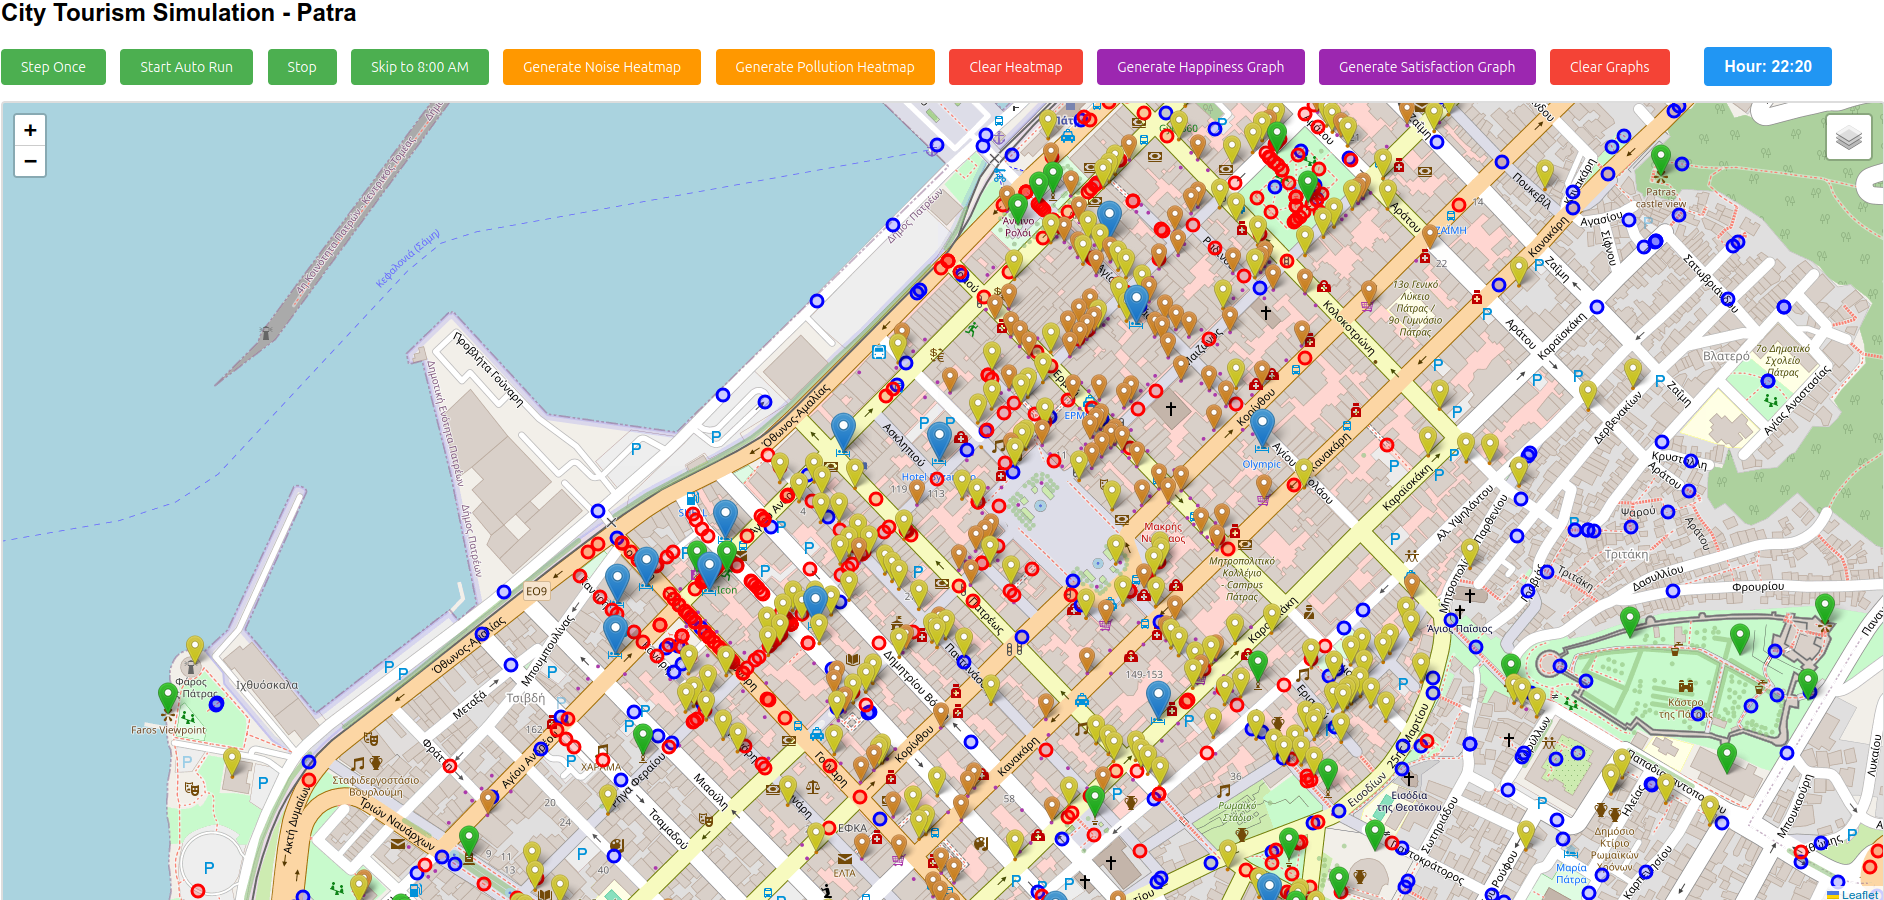
\includegraphics[width=\textwidth]{static/figures/map.png}
\caption{Χάρτης \en{Leaflet}}\label{map}
\end{figure}

\subsection{\en{Heatmaps} Θορύβου και Ρύπανσης}

Κατά την ενεργοποίηση \en{heatmap}, το \en{frontend} καλεί το
αντίστοιχο \en{endpoint} (\en{/heatmap/noise} ή
\en{/heatmap/pollution}) και λαμβάνει το πλέγμα τιμών μαζί με τα
γεωγραφικά όρια κάθε κελιού. Για κάθε κελί με μη-μηδενική τιμή
δημιουργείται ένα \en{L.rectangle} με χρώμα και διαφάνεια που
εξαρτώνται από την κανονικοποιημένη τιμή του κελιού σε σχέση με το
μέγιστο του πλέγματος.

Για τον θόρυβο χρησιμοποιείται χρωματική κλίμακα από κίτρινο (χαμηλές
τιμές) έως κόκκινο (υψηλές τιμές), ενώ για τη ρύπανση χρησιμοποιείται
κλίμακα καφέ αποχρώσεων. Η αδιαφάνεια \en{(fillOpacity)} κυμαίνεται
από 0.4 έως 0.8 ανάλογα με την τιμή, ώστε ο υποκείμενος χάρτης να
παραμένει ορατός. Κάθε ορθογώνιο κελί φέρει \en{popup} που εμφανίζει
την απόλυτη και κανονικοποιημένη τιμή.

\begin{figure}[H] \centering
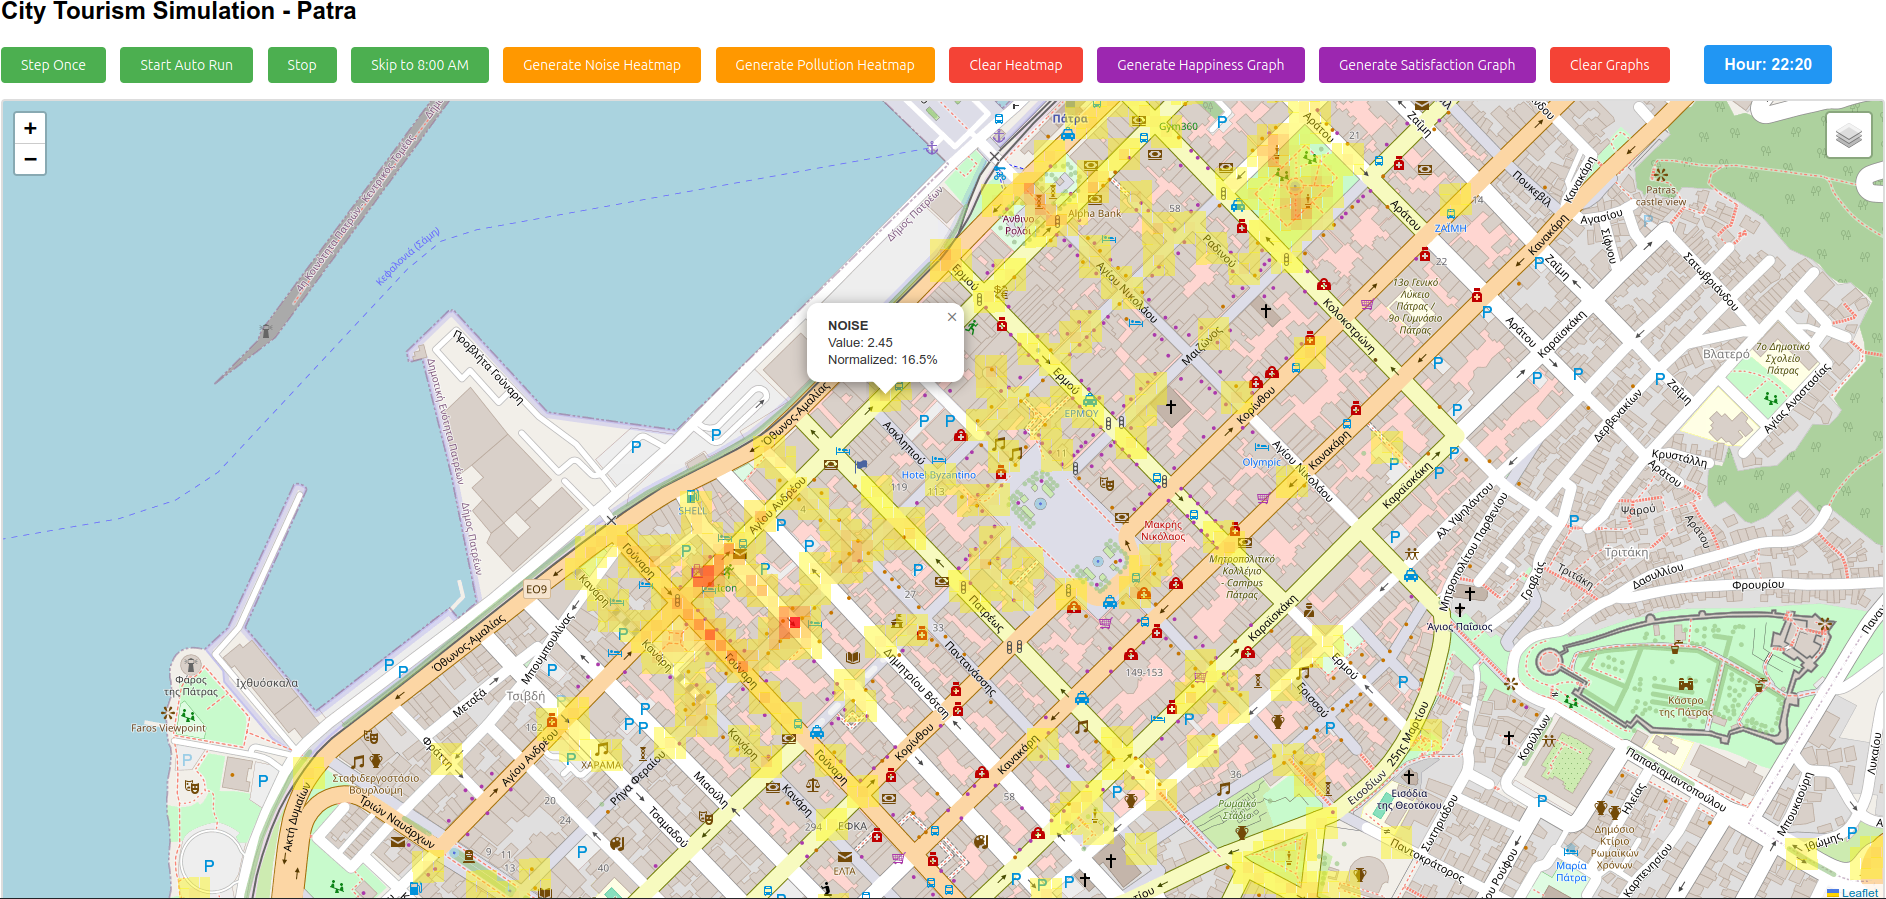
\includegraphics[width=\textwidth]{static/figures/noise_heatmap.png}
\caption{\en{Heatmap} Θορύβου}\label{heatmap}
\end{figure}

\subsection{\en{Charts} Κατανομής Ευτυχίας και Ικανοποίησης}

Τα γραφήματα κατανομών υλοποιούνται με \en{Chart.js} και εμφανίζονται
κάτω από τον χάρτη σε κρυφά \en{div containers} που γίνονται ορατά όταν
ο χρήστης ενεργοποιήσει το αντίστοιχο κουμπί. Κατά την ενεργοποίηση,
καλείται το \en{endpoint /distribution/happiness} ή
\en{/distribution/satisfaction} και τα δεδομένα αποδίδονται ως
ραβδόγραμμα \en{(bar chart)} με 10 \en{bins} στο διάστημα [0.0, 1.0].

Το γράφημα ευτυχίας χρησιμοποιεί μπλε χρωματισμό και εμφανίζει τον
αριθμό κατοίκων ανά εύρος τιμών ευτυχίας, ενώ το γράφημα ικανοποίησης
χρησιμοποιεί μωβ χρωματισμό για τους τουρίστες. Ο συνολικός αριθμός
πρακτόρων κάθε κατηγορίας εμφανίζεται ως τίτλος του γραφήματος. Εάν ο
χρήστης ζητήσει νέο γράφημα, το προηγούμενο καταστρέφεται πριν
δημιουργηθεί το νέο, αποφεύγοντας διπλότυπα \en{instances} του
\en{Chart.js}.

\begin{figure}[H] \centering
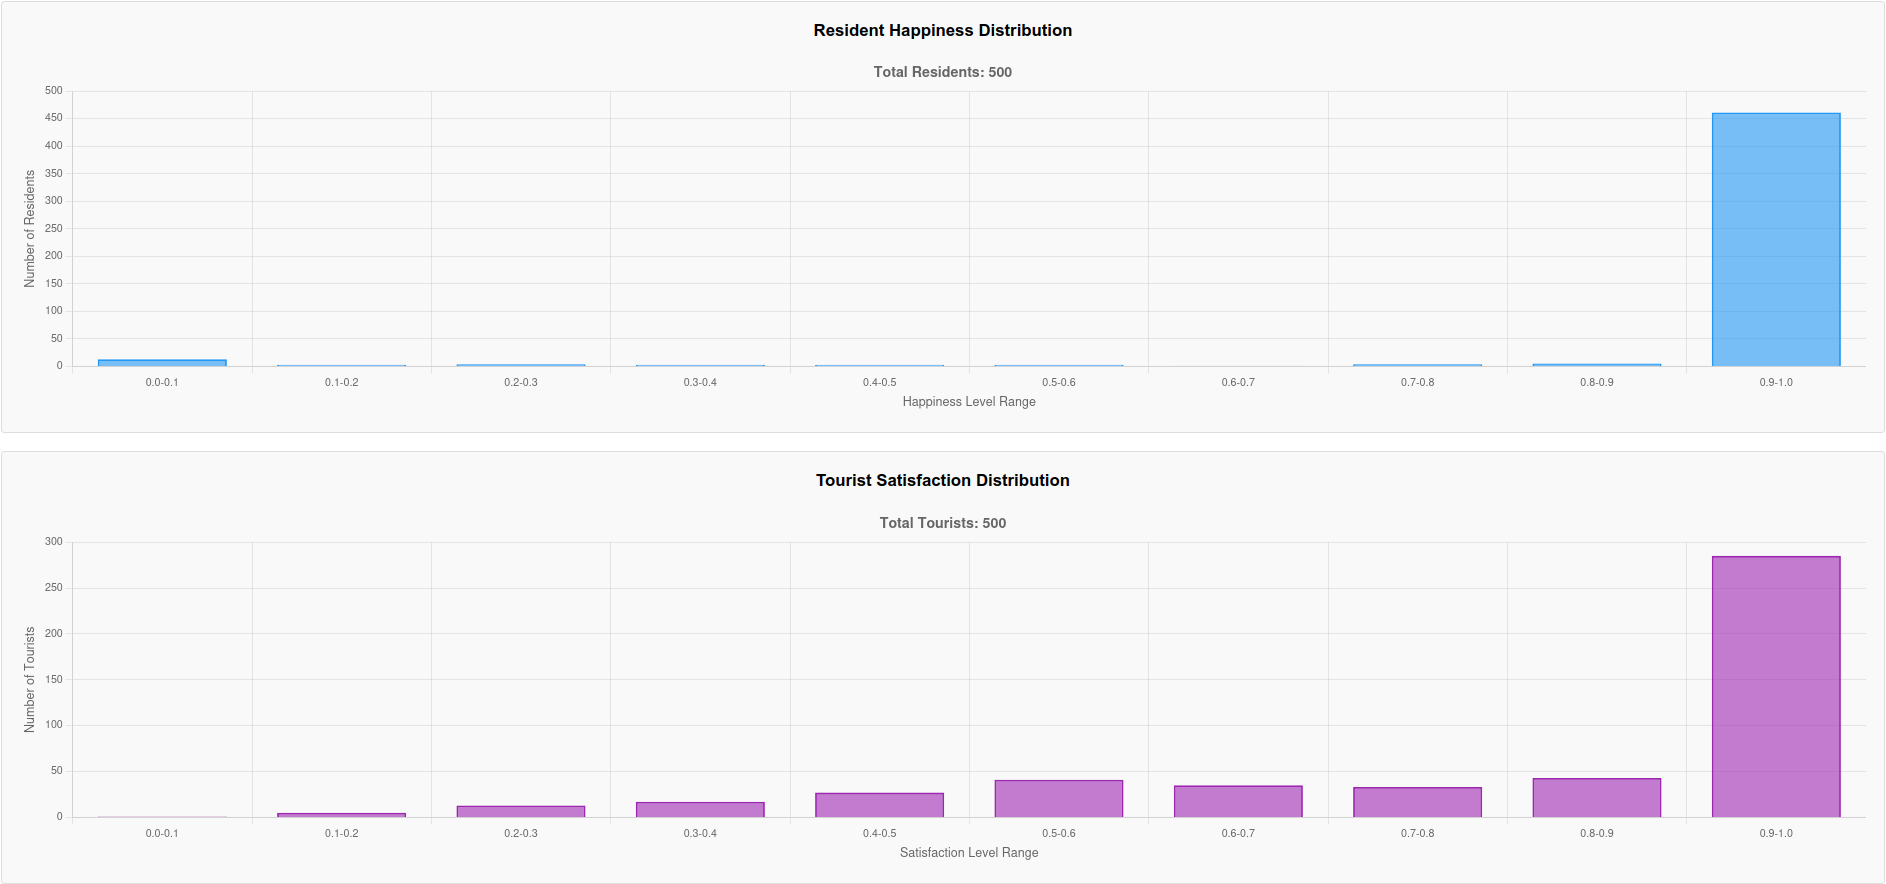
\includegraphics[width=\textwidth]{static/figures/charts.png}
\caption{\en{Charts} Κατανομής Ευτυχίας και Ικανοποίησης}\label{charts}
\end{figure}